\section{Design}\label{sec: Design}
In this section the design and decisions that where made to achieve it are discussed.

\subsection{Part 1 - Behavioral Modeling of a Seven-Segment Display}\label{sub: Behavioral Modeling of a Seven-Segment Display}
Verilog is used to describe a decoder that shall control a seven-segment display with two switches and one button. The given task is as followed:
\\
\\
In this part, you will simulate a pattern decoder using the buttons, switches, and a single seven-segment display.
Using switches, SW0 and SW1 as the pattern input, write a Verilog program that takes the binary input
combinations of the switches and displays the decimal value of the binary switch combination on the seven-segment
display. Table 1 shows the switch combinations with the expected output value on the seven-segment
display.

\begin{figure}[htbp]
	\centering
	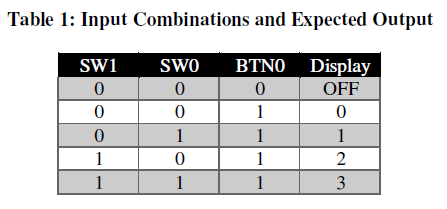
\includegraphics[width=0.6\textwidth]{01_images/Vivado_lab2_part1_table1.png}
	%\caption{Schematic directional coupler \cite{Vizmuller1995}}
	\label{fig: Vivado_lab2_part1_table1}
\end{figure}

As software package to implement the decoder in Verilog Vivado 2017.2 is used. 

\subsection{Part II - Hardware Implementation \& Modular Design}\label{sub: Hardware Implementation Modular Design}
For the second part a hierarchical design is achieved including the implementation and generation of a bit stream to use hardware or more specific the PYNQ development board. Therfore the folowing task is given:
\\
\\
In this part, you will modify your code from Part I. Instead of only using one button and one switch, you will
design your Verilog code to display on four seven-segment displays by pressing the four buttons on the PYNQ
board. Each seven-segment display will correspond to one button (i.e., BTN0 lights up the right-most seven-segment
display and BTN1 will light up the adjacent seven-segment display and so on). Make sure that when a
button is released, the corresponding seven-segment display turns OFF. Only one seven-segment display should
be on at any given time.
\\
\\
To realize the constrained file the PYNQ reference manual was used to allocate the right pins for the switches and buttons, figure \ref{fig: PYNQ_BasicIO} shows the basic I/O pins assignment of the PYNQ development board.
\begin{figure}[htbp]
	\centering
	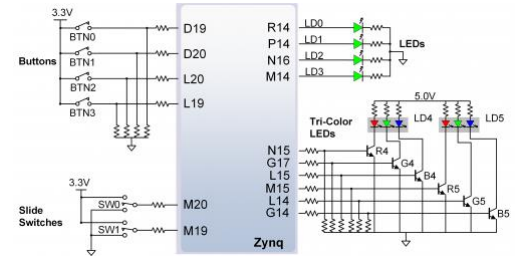
\includegraphics[width=0.6\textwidth]{01_images/PYNQ_BasicIO.png}
	\caption{Schematic PYNQ Basic I/O. \cite{PYNG_RM}}
	\label{fig: PYNQ_BasicIO}
\end{figure}
%
%The maximum current of the directional coupler can be calculated as follow

%
%The used schematic is shown in figure \ref{fig: Schematic directional coupler} which is based on two transformers T1 and T2.
%
%\begin{figure}[htbp]
%	\centering
%	\includegraphics[width=\textwidth]{images/RFDG_p107_Coupler_Schematic.jpg}
%	\caption{Schematic directional coupler \cite{Vizmuller1995}}
%	\label{fig: Schematic directional coupler}
%\end{figure}
%
%As design a multi core ferrite made of Material 67 was chosen as basis to wind the coupler.
%\begin{itemize}
% \item \begin{description}
% 	\item [Mfr.:] Fair-Rite
% 	\item [Mfr. \#:] 2867000102
% 	\item [Description] Ferrite Toroids / Ferrite Rings 67 MULIT APERTURE 13.3mm 13.4mm 7.5mm
% \end{description}
%\end{itemize}
%The wire used to wrap the coupler is AWG 22 magnet wire. According to tables on the Internet there is a current rating range from 0.9 A up to 5 A, so it is not unreasonable to not assume that it will be ok to operate the coupler on 50 W power.
%\begin{itemize}
%	\item \begin{description}
%	\item[Mfr.:] CNC Tech
%	\item[Mfr. \#:] 600222
%	\item [Description] MW35-C HY 22AWG 1KG/2.2LBS SPOOL
%	\item [Digi-Key Part Number]	1175-1687-ND	
%\end{description}
%\end{itemize}
%
%From the the Fair-Rite web page following information is available shown in figure \ref{fig: 67 Material Ferrite Toroid } which shows the complex permeability vs frequency and permeability vs temperature.
%
%\begin{figure}[htbp]
%	\centering
%	\begin{subfigure}[b]{0.4\textwidth}
%		\centering
%		\includegraphics[width=\textwidth ]{images/Ferrite-Torroit-67-Perm-vs-Freq2.jpg}
%		\caption{67 Material Characteristics}
%	\end{subfigure}
%	\begin{subfigure}[b]{0.4\textwidth}
%		\centering
%		\includegraphics[width=\textwidth]{images/Ferrite-Torroit-67-Perm-vs-Temp.jpg}
%		\caption{67 Material Characteristics}
%	\end{subfigure}
%	\caption{67 Material Ferrite Toroid \cite{fair_rite_07182018} }
%	\label{fig: 67 Material Ferrite Toroid }
%\end{figure}
%
%The steps to apply the windings are shown in figure \ref{fig: Directional coupler construction }.
%\begin{description}
%	\item[Step 1] On each hole of the multi toroid 9 windings are winded with magnet wire AWG 22. On one side, does not matter which one due to symmetry, the wires are desolated with sand paper and twisted together.
%	\item[Step 2] The two open wire ends are desolated with sand paper and crossed.
%	\item[Step 3] A single wire is first desolated on one side and pushed trough one of the openings, it does not matter which is chosen due to symmetry. and twisted together with the already existing wire that was crossed in the previous step.
%	\item[Step 4] Do the same as in step 3 on the opposite hole and desolate both wires. The finished coupler is shown in Step 4.
%\end{description}
%\begin{figure}[htbp]
%	\centering
%	\begin{subfigure}[b]{0.4\textwidth}
%		\centering
%		\includegraphics[width=0.4\textwidth, angle=270]{images/DC_Construction_001}
%		\caption{Step 1}
%	\end{subfigure}
%	\begin{subfigure}[b]{0.4\textwidth}
%		\centering
%		\includegraphics[width=0.8\textwidth]{images/DC_Construction_002}
%		\caption{Step 2}
%	\end{subfigure}
%	\begin{subfigure}[b]{0.4\textwidth}
%	\centering
%	\includegraphics[width=0.6\textwidth, angle=90]{images/DC_Construction_003}
%	\caption{Step 3}
%	\end{subfigure}
%	\begin{subfigure}[b]{0.4\textwidth}
%	\centering
%	\includegraphics[width=0.4\textwidth, angle=270]{images/DC_Construction_004}
%	\caption{Step 4}
%\end{subfigure}
%	\caption{Directional coupler construction }
%	\label{fig: Directional coupler construction }
%\end{figure}
%
%\newpage
%\subsection{RF Trace width 2 and 4 layer board design} \label{sub: RF Trace width 2 and 4 layer board design}
%\begin{figure}[htbp]
%	\centering
%	\begin{subfigure}[b]{0.4\textwidth}
%		\centering
%		\includegraphics[width=\textwidth]{images/pcbtracewidth_60mils_h}
%		\caption{2 layer board substrate height 60 mil}
%	\end{subfigure}
%	\begin{subfigure}[b]{0.4\textwidth}
%		\centering
%		\includegraphics[width=\textwidth]{images/pcbtracewidth_10mils_h}
%		\caption{4 layer board substrate height 10 mil}
%	\end{subfigure}
%	\caption{RF Trace width}
%\end{figure}
%
%Is used as power detector
%s
%\begin{figure}[htbp]
%	\centering
%	\includegraphics[width=\textwidth]{images/LTC5507_RF_POWER_DETECTOR}
%	\caption{Schematic and capacitor formula of the LTC5507 RF power detector}
%\end{figure}
%
%\newpage
%\subsection{Impedance matching strategy} \label{sub: Impedance matching strategy}
%The impedance matching needs to be based on the Standing Wave Ratio (SWR) measurement that is derived form the incident voltage wave and the reflected voltage wave.???
%
%\begin{equation}
%|\Gamma_0| = \frac{|V^-|}{|V^+|}
%\end{equation}
%
%\begin{equation}
%SWR = \frac{|V_{max}|} {|V_{min}|} = \frac{1+|\Gamma_0|} {1-|\Gamma_0|}
%\end{equation}
%The minimum voltage divided by the maximum voltage results in the reflection coefficient.
%
%
%
%Diodes - Variable Capacitance (Varicaps, Varactors)  not used because of temperature influence.
% 
% 
%\subsection{Link budget RF detector} \label{sub: Link budget RF detector}
%A link budget was made to figure out the necessary attenuation so that the requirements of a power range of 1 W to 50 W is met. The link budget, see figure \ref{fig: Link budget RF power detector}, shows that an attenuation of 13 dB is required. 
%
%For attenuation a PI-attenuator can be used which is composed out of resistors. Resistors aren't an issue here because the attenuator is not placed in the main RF path instead between coupled port of the directional coupler and RF power detector. For a impedance of Z0 equal to 50 $\Omega$ and $G_{Atten}$ equal to 13 dB, R1 is equal to 78.8447 $\Omega$ and R2 is equal to 106.0741 $\Omega$.
%\begin{verbatim}
%% IN                       OUT
%% Z0 ----+-----/\/\/\-----+------ Z0
%%        |       R2       |  
%%        >                >
%%        >  R1            > R1
%%        >                >
%%        |                |
%%       ---              ---
%%       ///              ///
%\end{verbatim}
%
%\begin{figure}[htbp]
%	\centering
%	\includegraphics[width=\textwidth]{images/linkbudget_rf_detector_002.jpg}
%	\caption{Link budget RF power detector}\label{fig: Link budget RF power detector}
%\end{figure}
%
%\subsection{Series-Shunt PIN Diode RF Switch} \label{sub: Series-Shunt PIN Diode RF Switch}
%As RF switch a PIN Diode was chosen. The decision was based on the diodes capability of temperature handling, the frequency range, and the power. A good deal of information does the document THE PIN DIODE CIRCUIT DESIGNERS’ HANDBOOK from Microsemi in Watertown, MA provide, which is saved under the path ../01\_Documentation/04\_PIN\_Diode. 
%
%The function of a series-shunt PIN Diode can be explained as if the switch is closed the a negative voltage bias is applied to the bias port so that the series diode is (reversed biased) conducting and the shunt diode is (forward biased) and not conducting. To have the switch open the voltage polarity is positive applied. The described behavior is shown in figure \ref{fig: Series-shunt PIN diode switch measurements 001}. The x-axis is the applied bias voltage. The left y-axis is the power in dBm for either the input signal applied from the signal generator or the output signal measured with the spectrum analyzer. The left y-axis is the current drawn from the power supply in mA.   
%
%\begin{figure}[htbp]
%	\centering
%	\includegraphics[width=\textwidth]{../04_PIN_Diode/07312018_PIN_Diode_SMP1352_001.pdf}
%	\caption{Series-shunt PIN diode switch measurements 001.}\label{fig: Series-shunt PIN diode switch measurements 001}
%\end{figure}
%
%\begin{figure}[htbp]
%	\centering
%	\includegraphics[width=\textwidth]{../04_PIN_Diode/08012018_PIN_Diode_SMP1352_002.pdf}
%	\caption{Series PIN diode switch measurements 002.}\label{fig: Series PIN diode switch measurements 002}
%\end{figure}


